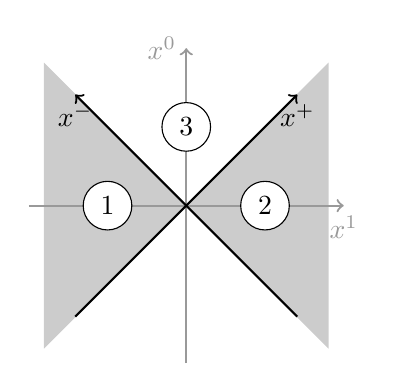
\begin{tikzpicture}
%light cone
\filldraw[black!20] (-1.8,1.8) -- (-1.8,-1.8) -- (1.8,1.8)  -- (1.8,-1.8) -- cycle;
%axes
\draw[->,gray!80,thick] (-2,0) -- (2,0) node[below] {$x^1$};
\draw[->,gray!80,thick] (0,-2) -- (0,2) node[left] {$x^0$}; 
\draw[->,thick] (1.41,-1.41) -- (-1.41,1.41) node[below] {$x^-$};
\draw[->,thick] (-1.41,-1.41) -- (1.41,1.41) node[below] {$x^+$};
%text
\draw (0,1) node[circle,fill=white,draw=black] {$3$};
\draw (-1,0) node[circle,fill=white,draw=black] {$1$};
\draw (1,0) node[circle,fill=white,draw=black] {$2$};
\end{tikzpicture}